
%(BEGIN_QUESTION)
% Copyright 2004, Tony R. Kuphaldt, released under the Creative Commons Attribution License (v 1.0)
% This means you may do almost anything with this work of mine, so long as you give me proper credit

This is a schematic diagram of a {\it Y-connected} three-phase generator (with the rotor winding shown):

$$\includegraphics[width=15.5cm]{i02294x01.eps}$$

How much AC voltage will appear between any two of the lines ($V_{AB}$, $V_{BC}$, or $V_{AC}$) if each stator coil inside the alternator outputs 277 volts?  Draw a phasor diagram showing how the phase (winding) and line voltages relate.

\vskip 10pt

How much AC current will each of the lines ($I_A$, $I_B$, or $I_C$) conduct to a load (not shown) if each stator coil inside the alternator outputs 17 amps of current to a load?

\vskip 10pt

How much power will be delivered to a load given the stator coil voltages and currents described above?

\vskip 20pt \vbox{\hrule \hbox{\strut \vrule{} {\bf Suggestions for Socratic discussion} \vrule} \hrule}

\begin{itemize}
\item{} Explain how you may double-check your quantitative answer(s) with a high degree of confidence (i.e. something more rigorous than simply re-working the problem again in the same way).
\item{} Explain the purpose of the {\it rotor winding} shown in the diagram.  Does this winding generate power or receive power from an external source?
\item{} Explain the purpose of the {\it DC excitation} shown in the diagram.  What would the generator do without this DC circuit in place and functioning?
\end{itemize}

\underbar{file i02294}
%(END_QUESTION)





%(BEGIN_ANSWER)

Phase voltage = 277 volts AC (given)

Line voltage = $V_{AB} = V_{BC} = V_{AC} = V_{phase} \sqrt{3} = $ 480 volts AC

$$\includegraphics[width=15.5cm]{i02294x02.eps}$$

\vskip 10pt

Phase current = 17 amps AC (given)

Line current = $I_{A} = I_{B} = I_{A} = I_{phase} = $ 17 amps AC

\vskip 10pt

Total load power = total source power = $3 I_{phase} V_{phase} = I_{line} V_{line} \sqrt{3} = $ 14.13 kW

%(END_ANSWER)





%(BEGIN_NOTES)

Students will quickly discover that $\sqrt{3}$ is the ``magic number'' for practically all balanced three-phase circuit calculations!

It should be noted that although the {\it magnitudes} of $V_{AB}$, $V_{BC}$, and $V_{AC}$ are equal, their phasor angles are most definitely not.  Therefore,

$$V_{AB} = V_{BC} = V_{AC} \hbox{\hskip 20pt Scalar values equal}$$

$${\bf V_{AB}} \neq {\bf V_{BC}} \neq {\bf V_{AC}} \hbox{\hskip 20pt Phasors unequal}$$

%INDEX% Electronics review: 3-phase voltage/current/power calculation

%(END_NOTES)


